\documentclass{standalone}
\usepackage{tikz}
%------------tikz Setup------------

\tikzstyle{ball} = [circle,shading=ball, ball color=black,
    minimum size=1mm,inner sep=1.3pt]
\tikzstyle{miniball} = [circle,shading=ball, ball color=black,
    minimum size=1mm,inner sep=0.5pt]
\tikzstyle{mminiball} = [circle,shading=ball, ball color=black,
    minimum size=0.6mm,inner sep=0.1pt]
\usetikzlibrary{arrows.meta}
\usetikzlibrary{angles, quotes}
\tikzset{>={Latex[length=2mm,width=1.5mm]}}
\tikzset{->-/.style={decoration={markings, mark=at position #1 with
  {\arrow{>}}},postaction={decorate}}}
\usetikzlibrary{decorations.pathmorphing}
\usetikzlibrary{decorations.pathreplacing}
\usetikzlibrary{arrows.meta,calc}
\usetikzlibrary{bending}
\usetikzlibrary{decorations.markings,shapes.geometric}
\tikzset{->-/.style={decoration={markings, mark=at position #1 with
  {\arrow{>}}},postaction={decorate}}}
\tikzset{-|-/.style={decoration={markings, mark=at position #1 with
  {\arrow{stealth}}},postaction={decorate}}}
\tikzset{movearrow/.style 2 args ={
        decoration={markings,
    mark= at position {#1} with {\arrow{#2}} ,
        },
        postaction={decorate}
    }
}


\begin{document}
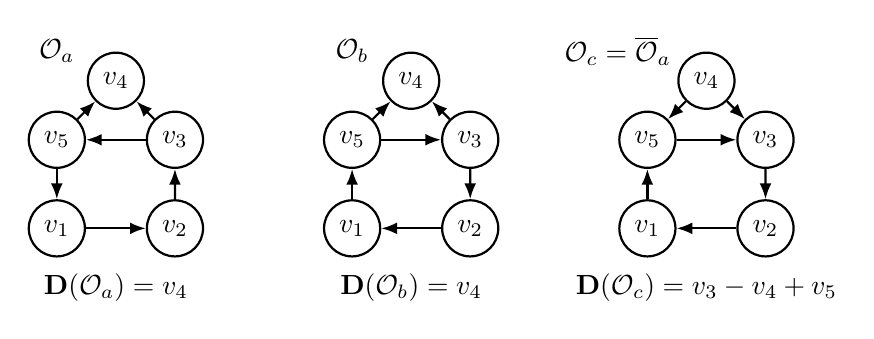
\begin{tikzpicture}[thick,main/.style = {draw, circle}]
\begin{scope}[scale=0.75]
    \node (o) at (0,3) {$\mathcal{O}_a$};
    \node (l) at (1,-1) {$\textbf{D}(\mathcal{O}_a)=v_4$};
    \node[main] (1) at (0,0) {$v_1$}; 
    \node[main] (2) at (2,0) {$v_2$}; 
    \node[main] (3) at (2,1.5) {$v_3$};
    \node[main] (4) at (1,2.5) {$v_4$};
    \node[main] (5) at (0,1.5) {$v_5$};
    \draw[thick,->] (1) to (2);
    \draw[thick,->] (2) to (3);
    \draw[thick,->] (3) to (5);
    \draw[thick,->] (5) to (1);
    \draw[thick,->] (3) to (4);
    \draw[thick,->] (5) to (4);
\end{scope}
\begin{scope}[scale=0.75,xshift=5cm]
    \node (o) at (0,3) {$\mathcal{O}_b$};
    \node (l) at (1,-1) {$\textbf{D}(\mathcal{O}_b)=v_4$};
    \node[main] (1) at (0,0) {$v_1$}; 
    \node[main] (2) at (2,0) {$v_2$}; 
    \node[main] (3) at (2,1.5) {$v_3$};
    \node[main] (4) at (1,2.5) {$v_4$};
    \node[main] (5) at (0,1.5) {$v_5$};
    \draw[thick,->] (2) to (1);
    \draw[thick,->] (3) to (2);
    \draw[thick,->] (5) to (3);
    \draw[thick,->] (1) to (5);
    \draw[thick,->] (3) to (4);
    \draw[thick,->] (5) to (4);
\end{scope}
\begin{scope}[scale=0.75,xshift=10cm]
    \node (o) at (-0.5,3) {$\mathcal{O}_c=\overline{\mathcal{O}}_a$};
    \node (l) at (1,-1) {$\textbf{D}(\mathcal{O}_c)=v_3-v_4+v_5$};
    \node[main] (1) at (0,0) {$v_1$}; 
    \node[main] (2) at (2,0) {$v_2$}; 
    \node[main] (3) at (2,1.5) {$v_3$};
    \node[main] (4) at (1,2.5) {$v_4$};
    \node[main] (5) at (0,1.5) {$v_5$};
    \draw[thick,->] (2) to (1);
    \draw[thick,->] (3) to (2);
    \draw[thick,->] (5) to (3);
    \draw[thick,->] (1) to (5);
    \draw[thick,->] (4) to (3);
    \draw[thick,->] (4) to (5);
\end{scope}
\end{tikzpicture}
\end{document}